% Biên dịch (XeLaTeX, cần fontspec): build ngoài thư mục doc/ rồi chỉ chép PDF vào doc/, ví dụ
% latexmk -xelatex -interaction=nonstopmode -halt-on-error -outdir=<thư mục tạm> doc/bao_cao_khoa_hoc_he_thong_zkstego_vi.tex
\documentclass[11pt,a4paper]{article}
\usepackage[margin=22mm,headheight=16pt]{geometry}
\usepackage{fontspec}
\setmainfont{Times New Roman}
\setmonofont{Consolas}
\usepackage{graphicx,booktabs,tabularx,array}
\usepackage{amsmath,amssymb}
\usepackage{xcolor,tikz}
\usetikzlibrary{arrows.meta,positioning,shapes.geometric,fit,calc}
\usepackage{hyperref,caption,float,listings,enumitem,fancyhdr}
\hypersetup{colorlinks=true,linkcolor=blue!50!black,urlcolor=blue!55!black,
  pdftitle={Hệ thống nhúng payload ZK vào H.264/CAVLC},
  pdfauthor={Báo cáo kỹ thuật dựa trên mã nguồn và kết quả benchmark của dự án}}
\setlength{\parskip}{0.42em}
\setlength{\parindent}{1em}
\setlist{nosep,leftmargin=2em}
\pagestyle{fancy}
\fancyhf{}
\lhead{ZK-Stego: H.264/CAVLC}
\rhead{Tài liệu kỹ thuật}
\cfoot{\thepage}
\renewcommand{\arraystretch}{1.14}
\setlength{\emergencystretch}{2em}
% Cho phép xuống dòng sau dấu gạch dưới trong tên tệp/định danh dài.
\let\origunderscore\_
\renewcommand{\_}{\origunderscore\allowbreak}
\captionsetup{font=small,labelfont=bf}
\lstset{basicstyle=\ttfamily\footnotesize,breaklines=true,frame=single,columns=fullflexible,
  showstringspaces=false,keywordstyle=\color{blue!55!black},commentstyle=\color{gray!70!black}}

\title{\textbf{Hệ thống nhúng payload mang bằng chứng ZK vào video H.264/CAVLC}}
\author{Tài liệu kỹ thuật dựa trên mã nguồn và artifact benchmark của dự án}
\date{25 tháng 9 năm 2026 \quad(cập nhật 3 tháng 10 năm 2026)}

\begin{document}
\maketitle

\noindent\fcolorbox{orange!70!black}{orange!6}{\parbox{\dimexpr\textwidth-2\fboxsep-2\fboxrule\relax}{\small
\textbf{Cập nhật 03/10/2026.} Báo cáo được sửa để khớp với hệ thống hiện tại:
(1) chỉ còn \emph{một lõi media native C++}; pipeline Python song song cũ và các benchmark SEC1--SEC10 đã bị gỡ khỏi repository ngày 03/10/2026, kết quả của chúng không còn là bằng chứng;
(2) kênh nhúng dùng \emph{giao thức v2}: khóa con HKDF-SHA256 cho lịch/tag/làm trắng, khung version \texttt{0x02}, tag HMAC-SHA256 cắt 16 byte, làm trắng bằng keystream HMAC, giao thức theo đoạn IDR có giới hạn bit mỗi IDR;
(3) mạch Groth16 có ràng buộc bit 0/1 (63,321 constraints, 513 public input) và Groth16 verify là bước bắt buộc sau trích xuất;
(4) \emph{toàn bộ số đo benchmark trong báo cáo được ghi ngày 24/09/2026 với giao thức v1 và mạch cũ}; chúng được giữ làm mốc tham chiếu và phải đo lại trước khi trích dẫn cho phiên bản hiện tại (mục \ref{sec:bench}).}}

\section{Kiến trúc hệ thống}
Hệ thống có ba lớp với trách nhiệm tách biệt. Lớp \emph{proof} (Python + circom/snarkjs) tạo proof Groth16 cho một message và secret. Lớp \emph{kênh xác thực} đóng gói payload vào một khung có tag HMAC và quyết định vị trí nhúng theo khóa. Lớp \emph{media} (native C++, \texttt{native/src/cavlc\_stream.cpp}) phân tích bitstream H.264 Baseline/CAVLC, liệt kê vị trí mang bit và lật dấu hệ số mà không đổi độ dài mã. Phía nhận chỉ cần video stego và khóa: trích xuất mù, kiểm tag HMAC, tách proof rồi bắt buộc xác minh Groth16. Camera không tạo proof cho từng frame; proof được tạo trước, còn video là kênh mang payload.

\begin{figure}[H]\centering
\resizebox{\textwidth}{!}{\begin{tikzpicture}[
  node distance=7mm and 8mm,
  box/.style={draw,rounded corners,align=center,minimum height=13mm,text width=34mm,fill=blue!5},
  app/.style={box,fill=green!7}, arr/.style={-{Latex[length=2mm]},thick}]
\node[app] (m) {Message $m$\\ secret $s$ 32 byte};
\node[app,right=of m] (proof) {Circom witness\\ Groth16 prover\\ proof nén 129 B};
\node[app,right=of proof] (pack) {Payload\\ $[\mathrm{len}_4][m][\pi_{129}]$};
\node[box,right=of pack] (frame) {Khung v2: \texttt{0x02}, len,\\ payload, tag HMAC 16 B;\\ XOR keystream};
\node[box,below=17mm of m] (cover) {Cover H.264\\ Annex-B, CAVLC};
\node[box,right=of cover] (native) {C++ native: parser,\\ ứng viên dấu T1,\\ lịch HMAC theo đoạn};
\node[box,right=of native] (stego) {Stego H.264\\ (lật dấu, độ dài\\ mã không đổi)};
\node[box,right=of stego] (extract) {Trích xuất mù\\ chỉ với khóa;\\ kiểm version + tag};
\node[app,right=of extract] (verify) {Unpack +\\ Groth16 verify\\ \textbf{bắt buộc}};
\draw[arr] (m)--(proof); \draw[arr] (proof)--(pack); \draw[arr] (pack)--(frame);
\draw[arr] (frame.south) -- ++(0,-5mm) -| (native.north);
\draw[arr] (cover)--(native); \draw[arr] (native)--(stego);
\draw[arr] (stego)--(extract); \draw[arr] (extract)--(verify);
\end{tikzpicture}}
\caption{Các khối ứng dụng và video của hệ thống hiện tại. Dữ liệu được nhúng trong residual H.264 của IDR; hệ thống không dùng SEI hay container làm nơi chứa payload.}
\label{fig:architecture}
\end{figure}
Hình \ref{fig:architecture} phân biệt proof với carrier: Groth16 tạo bằng chứng một lần cho message, còn C++ chỉ xử lý bitstream và không chạy prover trong vòng lặp camera. Cùng một giao thức theo đoạn được dùng cho file, job HTTP và luồng WebSocket; tag HMAC hợp lệ chỉ chứng minh payload đến từ người có khóa và không bị sửa, \emph{không} thay cho bước Groth16 verify.

\begin{table}[H]\centering\small
\caption{Thành phần và hợp đồng dữ liệu chính (mã nguồn tại thời điểm 03/10/2026).}
\begin{tabularx}{\textwidth}{p{3.3cm}p{4.0cm}X}
\toprule Khối & Đầu vào & Đầu ra / trách nhiệm\\\midrule
Circom/snarkjs (\texttt{src/zk\_proof.py}) & $m$, $s$, artifact mạch & Witness, proof Groth16 BN254, nén 129 byte; verify chỉ chấp nhận khi snarkjs thoát 0 và in \texttt{OK!}.\\
Payload packer & Message, proof bytes & 4 byte độ dài big-endian, message, proof nén 129 byte.\\
Khung xác thực v2 & Payload, khóa 32 byte & HKDF tách khóa con; khung \texttt{[0x02][len 2B][payload][tag 16B]}; bit khung XOR keystream.\\
Annex-B/NAL reader & Byte stream H.264 & NAL unit, header, EBSP/RBSP; reader tăng dần nhận start code vắt qua chunk.\\
CAVLC parser + bộ thu ứng viên & IDR I-slice Baseline/CAVLC & Mỗi khối residual một ứng viên: dấu trailing-one đầu tiên, kèm offset bit RBSP.\\
Lịch + patcher theo đoạn & Ứng viên, bit đã làm trắng, khóa lịch & Chọn tối đa \texttt{max\_bits\_per\_IDR} vị trí mỗi đoạn SPS+PPS+IDR, sửa bit dấu, dựng lại EBSP/Annex-B.\\
Trích xuất mù + verify & Stego, khóa & Payload đã qua HMAC; job verify unpack rồi Groth16 verify bắt buộc.\\
\bottomrule
\end{tabularx}
\end{table}
Ngoài các khối trên, \texttt{src/native\_blind\_contract.py} là bản tham chiếu Python của lịch/khung (có test vector chéo ngôn ngữ với C++), không phải một đường media thứ hai.

\section{Benchmark và kết quả chính}\label{sec:bench}
Phần này được đưa lên trước phần giải thích mã hóa để người đọc biết ngay điều gì đã chạy được và bằng chứng đang ở trạng thái nào.

\subsection{Phạm vi bằng chứng sau cập nhật 03/10/2026}
\begin{table}[H]\centering\small
\caption{Nguồn bằng chứng và mức độ áp dụng cho phiên bản hiện tại.}
\begin{tabularx}{\textwidth}{p{4.2cm}p{3.0cm}X}\toprule
Nguồn & Thời điểm & Áp dụng cho bản hiện tại\\\midrule
Bộ test \texttt{run\_all.py} (12 phase) và CTest native & 03/10/2026 & Có, về chức năng: 126/126 test và CTest 1/1 qua trên host Windows; không gồm phase camera vật lý H1; không phải nghiệm thu edge.\\
Suite \texttt{\_new}: media run \texttt{20260924T150707Z\_2be60c}, \texttt{zkp\_new.json} & 24/09/2026 & Chưa: đo với giao thức v1 và mạch cũ; phải chạy lại.\\
Camera E2E \texttt{realtime\_camera\_runs\_20260924.json} (run 24) & 24/09/2026 & Chưa: giao thức v1, mạch cũ, trước bản sửa bộ đọc stdin native.\\
Benchmark SEC1--SEC10 của pipeline Python cũ & trước 03/10/2026 & Không: đã gỡ; chỉ còn trong lịch sử git, không được trích dẫn.\\
\bottomrule\end{tabularx}
\end{table}
Hai thay đổi ngày 03/10/2026 làm số đo cũ không còn đại diện trực tiếp: giao thức v2 thêm HKDF và làm trắng bit (thay đổi chi phí và vị trí nhúng; v2 không đọc được stego v1), và mạch thêm ràng buộc bit (số constraint đổi, proof theo khóa cũ không verify với khóa hiện tại). Các số dưới đây vì vậy là \emph{mốc tham chiếu lịch sử}.

\subsection{Thiết kế phép đo (suite \texttt{\_new}, 24/09/2026)}
Tập thử gồm 9 clip Y4M (Akiyo, City, Coastguard, Container, Deadline, Football, Foreman, Foreman 300-frame, Hall Monitor), mỗi clip ở 352$\times$288, 640$\times$480 và 1280$\times$960: 27 cấu hình, chỉ 30 frame đầu mỗi cấu hình. Encoder là FFmpeg 8.0.1/libx264 Constrained Baseline, CAVLC, QP 22, GOP=1/all-intra, không B-frame, một thread và một slice/IDR. Hai cỡ lớn được phóng từ nguồn CIF nên là stress test phân giải, không phải nội dung camera native HD. Chỉ \texttt{foreman\_cif.y4m} được lưu trong repository, nên clone mới tái tạo 3 thay vì 27 cấu hình. Host: Windows, Python 3.12.10; JSON ghi hash của tệp native đã dùng.

Theo mã \texttt{benchmark/media\_benchmark\_new.py}, mỗi cấu hình nhúng một payload thử 33 byte (không phải proof Groth16) với giới hạn 4096 bit/IDR. Payload nhỏ nên vừa trong IDR đầu: trong run này 29/30 frame của mỗi cấu hình không bị nhúng làm thay đổi. Một cấu hình qua gate khi đo được capacity, embed thành công, FFmpeg strict decode, trích xuất mù đúng khóa và khóa sai bị từ chối; ở run 24/09 điều kiện ``từ chối'' là mã thoát khác 0, còn mã hiện tại chặt hơn (mã thoát 2 kèm thông báo lỗi xác thực).

\begin{table}[H]\centering\small
\caption{Số đo đại diện của file pipeline (giao thức v1, 24/09/2026). Median tính trong từng nhóm 9 clip cùng độ phân giải.}
\begin{tabular}{lrrr}\toprule
Chỉ số & 352$\times$288 & 640$\times$480 & 1280$\times$960\\\midrule
Median output FPS & 215.23 & 66.96 & 12.95\\
Median RSS tiến trình native embed (MiB) & 9.70 & 17.11 & 45.82\\
Median source-to-stego PSNR-Y (dB) & 43.77 & 45.17 & 46.81\\
Số cấu hình qua gate & 9/9 & 9/9 & 9/9\\
\bottomrule\end{tabular}
\end{table}
Output FPS bằng 30 frame chia thời gian embed native; nó không bao gồm capture camera, encode hay thời gian scan capacity. RSS là peak lấy mẫu mỗi 5 ms của tiến trình native embed, không phải toàn bộ ứng dụng và có thể bỏ lỡ spike ngắn. Trung vị giảm từ 215.23 xuống 12.95 FPS khi tăng từ 352$\times$288 lên 1280$\times$960; kết quả không hỗ trợ kết luận đạt realtime 30 FPS ở mọi độ phân giải.

\begin{figure}[H]\centering
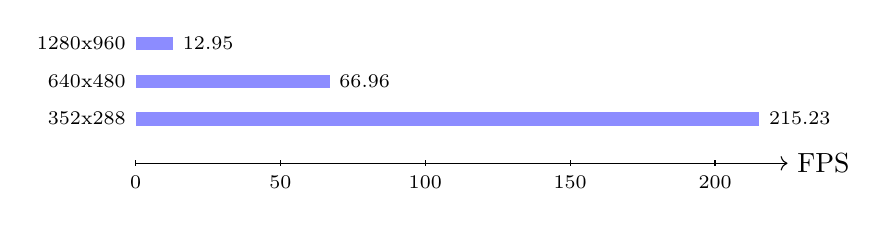
\begin{tikzpicture}[x=0.92cm,y=0.48cm]
\draw[->] (0,0)--(9,0) node[right]{FPS};
\foreach \x/\lab in {0/0,2/50,4/100,6/150,8/200}{
  \draw (\x,0.08)--(\x,-0.08) node[below]{\scriptsize \lab};}
\foreach \y/\name/\v/\w in {1/352x288/215.23/8.61,2/640x480/66.96/2.68,3/1280x960/12.95/0.52}{
  \node[left] at (0,\y+0.18){\scriptsize \name};
  \fill[blue!45] (0,\y)--(\w,\y)--(\w,\y+0.35)--(0,\y+0.35)--cycle;
  \node[right] at (\w,\y+0.18){\scriptsize \v};}
\end{tikzpicture}
\caption{Median output throughput theo độ phân giải trong 27 case file pipeline (giao thức v1). Cột 352$\times$288 vượt mốc 200 và số 215.23 được ghi cạnh cột.}
\label{fig:fps-resolution}
\end{figure}
Đây là phép đo embed offline trên đoạn H.264 đã encode, không phải đo end-to-end từ cảm biến. Ở 640$\times$480, median 66.96 FPS cao hơn mục tiêu 30 trên clip ngắn; ở 1280$\times$960, median 12.95 FPS thấp hơn mục tiêu. Kết luận hợp lý là throughput phụ thuộc mạnh vào độ phân giải và nội dung, chưa thể tuyên bố realtime tổng thể.

\begin{table}[H]\centering\small
\caption{Tóm tắt chất lượng ảnh và kiểm tra chức năng (run \texttt{20260924T150707Z\_2be60c}, giao thức v1).}
\begin{tabular}{p{6.2cm}p{3cm}p{4.8cm}}\toprule
Đại lượng & Kết quả & Cách đọc\\\midrule
Gate chức năng & 27/27 & Embed, strict decode, trích xuất mù đúng khóa, khóa sai bị từ chối.\\
Trung bình PSNR-Y source-to-stego & 46.84 dB & Gồm cả nén H.264 lossy và nhúng.\\
Trung bình SSIM source-to-stego & 0.99025 & Trung bình trên 27 cấu hình.\\
PSNR-Y thấp nhất trên frame bị sửa (cover-to-stego) & 32.76 dB & Hall Monitor, 1280$\times$960.\\
Cấu hình có frame sửa dưới 40 dB & 13/27 & 40 dB là mốc tham khảo, không phải gate chức năng.\\
Capacity scan & median 9.61 s; max 96.25 s & Tách biệt với embed time.\\
\bottomrule\end{tabular}
\end{table}
PSNR-Y đo sai khác cường độ luma theo dB; SSIM gần 1 khi cấu trúc hai ảnh tương tự. Source-to-stego gộp hai nguồn sai khác (nén và nhúng), còn cover-to-stego đối chiếu bản H.264 sạch với bản stego để cô lập ảnh hưởng nhúng. Vì chỉ một frame mỗi cấu hình bị sửa, PSNR trung bình cả clip che mất frame xấu; cần xem giá trị theo từng frame trong CSV. Run trước đó \texttt{20260924T144703Z\_840091} có 15/27 cấu hình dưới 40 dB (thấp nhất 34.13 dB) và chỉ được giữ để so sánh.

\begin{figure}[H]\centering
\begin{tikzpicture}[x=0.72cm,y=0.12cm]
\draw[->] (0,0)--(13,0) node[right]{dB};
\foreach \x/\lab in {0/30,2/35,4/40,6/45,8/50,10/55,12/60}{\draw (\x,0.6)--(\x,-0.6) node[below]{\scriptsize \lab};}
\draw[dashed,red!70!black] (4,-0.4)--(4,3.8) node[above,align=center]{\scriptsize 40 dB mốc tham khảo};
\node[left] at (0,1){\scriptsize frame sửa thấp nhất};
\fill[orange!70] (0,1)--(1.104,1)--(1.104,1.7)--(0,1.7)--cycle;
\node[right] at (1.104,1.35){\scriptsize 32.76};
\node[left] at (0,2.5){\scriptsize mean source-to-stego};
\fill[blue!55] (0,2.5)--(6.736,2.5)--(6.736,3.2)--(0,3.2)--cycle;
\node[right] at (6.736,2.85){\scriptsize 46.84};
\end{tikzpicture}
\caption{So sánh PSNR-Y trung bình toàn cấu hình với frame bị nhúng có chất lượng thấp nhất (giao thức v1).}
\label{fig:quality-gap}
\end{figure}
Khoảng cách giữa 46.84 dB và 32.76 dB cho thấy chỉ nhìn trung bình là chưa đủ. Hệ thống qua gate giải mã/khôi phục nhưng chưa đảm bảo ngưỡng chất lượng đồng đều trên từng frame. Với giao thức v2, vị trí nhúng thay đổi (lịch theo khóa con, bit đã làm trắng) nên phân bố chất lượng cần được đo lại chứ không suy ra từ bảng này.

\subsection{Proof system và luồng camera}
\begin{table}[H]\centering\small
\caption{Groth16 và PLONK trên cùng R1CS, witness và payload; mỗi hệ một trial (\texttt{zkp\_new.json}, 24/09/2026, \emph{mạch cũ 62,553 constraints, trước khi thêm ràng buộc bit} --- số liệu lịch sử).}
\begin{tabularx}{\textwidth}{p{3cm}p{2.4cm}p{2.4cm}X}\toprule
Chỉ số & Groth16 BN254 & PLONK KZG & Diễn giải\\\midrule
Witness & 433.93 ms & 422.59 ms & Có thời gian khởi động Node.\\
Prove & 2.581 s & 831.695 s & PLONK khoảng 13.86 phút ở phép đo này.\\
Verify & 848.36 ms & 1,013.60 ms & Một trial mỗi hệ, chưa có khoảng tin cậy.\\
Peak RSS prover & 1.12 GB & 19.82 GB & Lấy mẫu mỗi 10 ms, có thể hụt peak ngắn.\\
Proof serialized & 129 B nén / 808 B JSON & 2,251 B JSON & Bộ nén 129 byte chỉ có cho Groth16.\\
Setup/artifact & setup cục bộ, chưa audit & setup $\approx$668 s; proving key 21.88 GB & PLONK dùng transcript Powers-of-Tau cục bộ, power 18.\\
\bottomrule\end{tabularx}
\end{table}
Trong phép đo đơn này, Groth16 có proof nhỏ hơn và prove nhanh hơn đáng kể. Đây không phải so sánh thống kê và không gồm Halo2, STARK/RISC Zero hay Bulletproofs vì chưa có triển khai cùng mạch trong repository. Mạch hiện tại có 63,321 constraints (thêm ràng buộc bit, mục \ref{sec:groth16}); thời gian và bộ nhớ của nó chưa được đo lại. Số liệu SEC5 cũ (trộn một statement ZK-Schnorr khác với giá trị mô phỏng/trích tài liệu) không phải bằng chứng và đã bị loại.

\begin{table}[H]\centering\small
\caption{Một lần chạy camera E2E 60 giây có payload chứa proof Groth16 thật (run 24, 24/09/2026, giao thức v1, mạch cũ).}
\begin{tabular}{p{6cm}p{3cm}p{4.8cm}}\toprule
Đại lượng & Kết quả & Cách đọc\\\midrule
Frame ghi/giải mã & 450 / 450 & FFmpeg strict decode thành công.\\
Throughput & 7.608 FPS active; 7.331 gồm khởi động & Thấp hơn cổng 30 FPS: không đạt.\\
Proof và payload & Proof 129 B; verify đúng & Proof tạo trước capture, verify sau trích xuất.\\
Negative checks & Khóa sai và message sửa bị từ chối & Xác nhận đúng payload/statement trong lần chạy.\\
PSNR-YUV420 toàn video / frame sửa thấp nhất & 65.23 / 46.78 dB & Mean SSIM luma 0.999928.\\
Process-tree peak RSS & 188.84 MB & Gồm API, FFmpeg và native; lấy mẫu mỗi 100 ms.\\
\bottomrule\end{tabular}
\end{table}
Run 24 chứng minh, ở giao thức v1, đường E2E camera (DirectShow 352$\times$288 $\rightarrow$ FFmpeg $\rightarrow$ WebSocket loopback TCP $\rightarrow$ native) đã truyền proof thật, trích xuất mù và verify sau capture. Tạo proof mất 4.016 s ngoài đường capture; verify mất 2.074 s sau trích xuất. Một chẩn đoán riêng trên cùng host cho thấy trong điều kiện đó chính nguồn camera chỉ cấp khoảng 7.5 frame/s, nên con số 7.608 FPS chưa quy được cho transport hay xử lý native. Đây là một run đơn trên host phát triển; nó không chứng minh ổn định lâu dài, realtime 30 FPS hay kết quả trên thiết bị edge.

\textbf{Ghi chú hiệu năng sau đo.} Ngày 02/10/2026 bộ đọc stdin và bộ đọc bit native được sửa (reader không chờ lấp đầy khối lớn trên pipe live, quét start code tuyến tính). Một lần embed live 1080p all-intra trên host phát triển giảm từ 30.1 s xuống 2.5 s. Đây là phép đo chức năng, không phải benchmark có kiểm soát; con số 7.608 FPS ở trên được đo \emph{trước} bản sửa và chưa được đo lại.

\section{Từ ảnh đến H.264: nhìn thấy từng bước}
\subsection{RGB, Y, Cb, Cr và lấy mẫu màu}
\begin{figure}[H]\centering
\resizebox{\textwidth}{!}{\begin{tikzpicture}[x=1mm,y=1mm]
\draw[rounded corners,fill=blue!12] (0,0) rectangle (46,32);
\fill[blue!24] (0,16) rectangle (46,32); \fill[green!22] (0,0) rectangle (46,16);
\draw[fill=gray!35] (4,11) rectangle (15,25); \draw[fill=brown!45] (24,6) rectangle (39,23);
\draw[fill=gray!65] (21,6) rectangle (42,8);
\node[below] at (23,-2){\small RGB scene};
\draw[-{Latex[length=2mm]},thick] (48,16)--(60,16) node[midway,above]{\scriptsize color transform};
\draw[fill=gray!68] (64,18) rectangle (101,42); \node[anchor=north west] at (66,40){\small Y};
\foreach \x in {0,1,...,9}{\draw[gray!50] (64+3.7*\x,18)--(64+3.7*\x,42);}
\foreach \y in {0,...,5}{\draw[gray!50] (64,18+4*\y)--(101,18+4*\y);}
\draw[fill=green!45] (71,-4) rectangle (98,14); \node[anchor=north west] at (73,12){\small Cb};
\foreach \x in {0,...,6}{\draw[green!60!black] (71+3.85*\x,-4)--(71+3.85*\x,14);}
\foreach \y in {0,...,3}{\draw[green!60!black] (71,-4+4.5*\y)--(98,-4+4.5*\y);}
\draw[fill=blue!38] (103,-18) rectangle (130,0); \node[anchor=north west] at (105,-2){\small Cr};
\foreach \x in {0,...,6}{\draw[blue!65] (103+3.85*\x,-18)--(103+3.85*\x,0);}
\foreach \y in {0,...,3}{\draw[blue!65] (103,-18+4.5*\y)--(130,-18+4.5*\y);}
\node[align=left,text width=56mm] at (166,13) {Y: độ sáng, giữ đầy đủ\newline
Cb: sai khác xanh--vàng\newline
Cr: sai khác đỏ--lục\newline
YUV 4:2:0: Cb/Cr mỗi mặt phẳng có một nửa chiều ngang và chiều dọc};
\end{tikzpicture}}
\caption{Minh họa tự dựng RGB được phân thành ba mặt phẳng. Độ phân giải mỗi mặt phẳng màu thực tế phụ thuộc pixel format; benchmark dùng YUV420.}
\label{fig:ycbcr}
\end{figure}
RGB mô tả màu theo ba thành phần đỏ, lục, lam; encoder thường chuyển sang biểu diễn luma/chroma. Với YUV420, mỗi mẫu Cb/Cr đại diện vùng 2$\times$2 pixel, vì mắt nhạy với độ sáng hơn sai khác màu. Frame 352$\times$288 do đó giữ mặt phẳng Y 352$\times$288, còn mỗi chroma plane là 176$\times$144 (một frame Y4M 4:2:0 gồm 101,376 + 25,344 + 25,344 = 152,064 byte dữ liệu). Hình này là sơ đồ giải thích, không phải frame benchmark.

\subsection{Macroblock, dự đoán và residual}
\begin{figure}[H]\centering
\resizebox{\textwidth}{!}{\begin{tikzpicture}[x=1mm,y=1mm]
\draw[rounded corners,fill=cyan!10] (0,0) rectangle (58,42);
\fill[blue!15] (0,20) rectangle (58,42); \fill[green!18] (0,0) rectangle (58,20);
\draw[fill=gray!35] (5,19) rectangle (19,34); \draw[fill=brown!40] (31,7) rectangle (52,27);
\draw[fill=gray!60] (28,7) rectangle (54,9);
\foreach \x in {0,...,4}{\draw[gray!70] (\x*14.5,0)--(\x*14.5,42);}
\foreach \y in {0,...,3}{\draw[gray!70] (0,\y*14)--(58,\y*14);}
\draw[red,very thick] (29,7) rectangle (43,21);
\node[below] at (29,-3){Frame chia thành macroblock 16$\times$16};
\draw[-{Latex[length=2mm]},thick] (59,21)--(71,21);
\node[draw,rounded corners,fill=yellow!10,align=center,text width=38mm,minimum height=16mm] (pred) at (92,21) {Dự đoán intra\newline hoặc từ frame tham chiếu};
\draw[-{Latex[length=2mm]},thick] (112,21)--(124,21);
\node[draw,rounded corners,fill=orange!10,align=center,text width=36mm,minimum height=16mm] (res) at (145,21) {Residual = pixel gốc\newline $-$ pixel dự đoán};
\draw[-{Latex[length=2mm]},thick] (165,21)--(177,21);
\node[draw,rounded corners,fill=blue!8,align=center,text width=42mm,minimum height=16mm] at (201,21) {Transform 4$\times$4\newline $\rightarrow$ quantize $\rightarrow$ CAVLC};
\end{tikzpicture}}
\caption{Macroblock là vùng ảnh được mã hóa cùng thông tin dự đoán và residual; ô đỏ là ví dụ vùng được phóng to.}
\label{fig:macroblock}
\end{figure}
Encoder không biến thẳng pixel thành bit. Nó hình thành dự đoán từ các mẫu \emph{đã tái tạo} (trước deblocking) của khối lân cận, trừ dự đoán khỏi block nguồn để lấy residual, biến đổi residual thành hệ số tần số, lượng tử hóa và cuối cùng entropy-code. Với all-intra, frame không tham chiếu frame trước; đường nhúng native chỉ mang dữ liệu trong IDR I-slice/CAVLC. Vì dự đoán intra dùng mẫu đã tái tạo, một lần lật dấu có thể lan truyền sai khác sang các khối giải mã sau trong cùng frame.

\subsection{Lượng tử hóa và bảng QP}
H.264 không bắt buộc một ma trận quantization duy nhất cho mọi block. QP xác định mức bước lượng tử hóa; scaling lists (nếu có) điều chỉnh theo tần số và loại block. Dưới đây là chu kỳ hệ số bước cơ sở chuẩn hóa theo QP, với $q=\lfloor QP/6\rfloor$, $r=QP\bmod 6$, và $Q_{step}=V_r\,2^q$; hệ số $V_r$ theo quan hệ QP trong \href{https://www.itu.int/dms_pubrec/itu-t/rec/h/T-REC-H.264-202606-I%21%21SUM-HTM-E.htm}{ITU-T H.264 phiên bản 16}. Đây là mô hình bước lượng tử để đọc QP, không thay thế phép biến đổi/rounding integer chính xác ở encoder.

\begin{table}[H]\centering\small
\caption{Hệ số bước lượng tử cơ sở theo phần dư QP modulo 6.}
\begin{tabular}{crrr}\toprule
$r=QP\bmod6$ & $V_r$ & QP mẫu & $Q_{step}$ chuẩn hóa\\\midrule
0 & 0.6250 & 0 & 0.6250\\
1 & 0.6875 & 1 & 0.6875\\
2 & 0.8125 & 2 & 0.8125\\
3 & 0.8750 & 3 & 0.8750\\
4 & 1.0000 & 4 & 1.0000\\
5 & 1.1250 & 5 & 1.1250\\
\bottomrule\end{tabular}
\end{table}
Khi QP tăng 6, bước cơ sở tăng gấp đôi; hệ số nhỏ dễ bị lượng tử về 0. Tham số encoder là \texttt{-qp 22} ($q=3$, $r=4$, bước cơ sở $1\times2^3=8$). Tuy vậy libx264 ở chế độ QP cố định hạ QP của I-frame theo \texttt{ip\_ratio=1.40}: trace slice header của demo cho QP slice $=22-3=19$. QP thực của từng slice/MB vì vậy phải đọc từ bitstream, không suy từ tham số dòng lệnh. Hệ số được sửa để nhúng nằm \emph{sau} lượng tử hóa, vì thay đổi trước bước này sẽ bị encoder ghi đè.

\begin{figure}[H]\centering
\resizebox{\textwidth}{!}{\begin{tikzpicture}[x=1mm,y=1mm]
\node[align=center] at (28,42){\small Residual sample};
\node[align=center] at (82,42){\small Coefficient sau transform};
\node[align=center] at (141,42){\small Sau lượng tử hóa (ví dụ)};
\foreach \r in {0,...,3}{\foreach \c in {0,...,3}{
  \pgfmathsetmacro{\x}{8+10*\c}\pgfmathsetmacro{\y}{22-10*\r}
  \draw[fill=blue!5] (\x,\y) rectangle ++(10,10);
  \ifnum\r=0 \ifnum\c=0 \node at (\x+5,\y+5){8};\else \node at (\x+5,\y+5){1};\fi
  \else \ifnum\r=1 \ifnum\c=0 \node at (\x+5,\y+5){-2};\else \node at (\x+5,\y+5){0};\fi
  \else \node at (\x+5,\y+5){0};\fi\fi
}}
\draw[-{Latex[length=2mm]},thick] (53,22)--(61,22);
\foreach \r in {0,...,3}{\foreach \c in {0,...,3}{
  \pgfmathsetmacro{\x}{66+10*\c}\pgfmathsetmacro{\y}{22-10*\r}
  \draw[fill=orange!8] (\x,\y) rectangle ++(10,10);
  \ifnum\r=0 \ifnum\c=0 \node at (\x+5,\y+5){32};\else \node at (\x+5,\y+5){4};\fi
  \else \ifnum\r=1 \ifnum\c=0 \node at (\x+5,\y+5){-8};\else \node at (\x+5,\y+5){0};\fi
  \else \node at (\x+5,\y+5){0};\fi\fi
}}
\draw[-{Latex[length=2mm]},thick] (111,22)--(120,22);
\foreach \r in {0,...,3}{\foreach \c in {0,...,3}{
  \pgfmathsetmacro{\x}{125+10*\c}\pgfmathsetmacro{\y}{22-10*\r}
  \draw[fill=green!8] (\x,\y) rectangle ++(10,10);
  \ifnum\r=0 \ifnum\c=0 \node at (\x+5,\y+5){4};\else \node at (\x+5,\y+5){1};\fi
  \else \ifnum\r=1 \ifnum\c=0 \node at (\x+5,\y+5){-1};\else \node at (\x+5,\y+5){0};\fi
  \else \node at (\x+5,\y+5){0};\fi\fi
}}
\node[below,align=center,text width=160mm] at (91,-21){Số liệu được dựng để minh họa phép chia và làm tròn, không phải trace từ file encode. Trong H.264 thật, encoder áp dụng integer transform, scaling factor, shift và rounding theo vị trí (libx264 còn dùng dead-zone, trellis, psy-RD); vì vậy không dùng phép chia 8 giản lược để tái tạo bit-exact.};
\end{tikzpicture}}
\caption{Ví dụ số học minh họa: một residual block tạo ra hệ số biến đổi, sau đó lượng tử hóa làm hệ số nhỏ trở thành 0.}
\label{fig:quant-example}
\end{figure}
Lượng tử hóa làm thưa ma trận coefficient để entropy coder mã hóa ít symbol hơn, đổi lại mất thông tin không khôi phục được. Hệ thống sửa dấu coefficient đã lượng tử hóa và không thay QP; vì vậy nó không thể khôi phục chi tiết đã mất từ bước nén.

\subsection{Cấu hình encode tái lập}
Benchmark gọi FFmpeg/libx264 trên Y4M (\texttt{benchmark/media\_benchmark\_new.py}). Phần chính của lệnh như sau:
\begin{lstlisting}[language=bash]
ffmpeg -i input.y4m -frames:v 30 \
  -vf scale=W:H:flags=lanczos,format=yuv420p \
  -c:v libx264 -preset ultrafast -tune zerolatency \
  -profile:v baseline -qp 22 -g 1 -bf 0 -threads 1 -pix_fmt yuv420p \
  -x264-params "keyint=1:min-keyint=1:scenecut=0:repeat-headers=1:slices=1:threads=1" \
  -f h264 output.h264
\end{lstlisting}
Các flag quyết định điều kiện benchmark, không phải quy tắc của mọi H.264. Constrained Baseline dùng CAVLC; \texttt{-g 1 -bf 0} tạo all-intra không B-frame; một thread/một slice là bắt buộc vì parser native chỉ nhận một slice mỗi frame bắt đầu ở MB 0 (multi-slice tự động của FFmpeg nằm ngoài hợp đồng hỗ trợ). GOP$>$1 vẫn xử lý được nhưng P-frame không mang ứng viên.

\section{NAL, slice và loại frame I/P/B}
\subsection{Từ Annex-B bytes đến NAL header}
Annex-B là cách đóng khung byte stream H.264 bằng start code 3 hoặc 4 byte; NAL parser là phần mềm tìm marker, tách NAL, đọc header và chuyển EBSP/RBSP. Đầu stream ví dụ: \texttt{00 00 00 01 67 ...} (SPS), \texttt{00 00 00 01 68 ...} (PPS), \texttt{00 00 01 06 ...} (SEI của x264), \texttt{00 00 01 65 ...} (IDR slice). Byte header có \texttt{forbidden\_zero\_bit}, \texttt{nal\_ref\_idc}, \texttt{nal\_unit\_type}; type 5 nhận diện IDR slice. Start code không phải là header NAL.

\begin{figure}[H]\centering
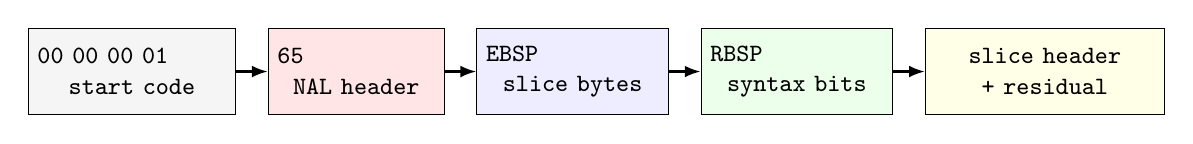
\begin{tikzpicture}[node distance=5mm and 4mm,cell/.style={draw,minimum height=11mm,align=center,font=\ttfamily\small},arr/.style={-{Latex[length=2mm]},thick}]
\node[cell,fill=gray!8,text width=24mm] (sc) {00 00 00 01\newline start code};
\node[cell,right=of sc,fill=red!10,text width=20mm] (hdr) {65\newline NAL header};
\node[cell,right=of hdr,fill=blue!7,text width=22mm] (ebsp) {EBSP\newline slice bytes};
\node[cell,right=of ebsp,fill=green!8,text width=22mm] (rbsp) {RBSP\newline syntax bits};
\node[cell,right=of rbsp,fill=yellow!10,text width=28mm] (slice) {slice header\\+ residual};
\draw[arr] (sc)--(hdr);\draw[arr] (hdr)--(ebsp);\draw[arr] (ebsp)--(rbsp);\draw[arr] (rbsp)--(slice);
\end{tikzpicture}
\caption{Giải phẫu NAL IDR minh họa. \texttt{0x65} có NAL type 5; payload sau header cần unescape trước khi đọc syntax.}
\label{fig:nal-format}
\end{figure}
Parser tìm start code, lấy NAL header, rồi bỏ byte emulation-prevention \texttt{03} để khôi phục RBSP; mọi offset bit của ứng viên tính trên RBSP. Lật một bit RBSP có thể tạo hoặc xóa mẫu \texttt{00 00 0x}, nên khi ghi lại NAL các byte EPB được tính lại: độ dài bit RBSP không đổi nhưng độ dài byte EBSP có thể lệch vài byte. Trong streaming, \texttt{AnnexBNalStreamReader} giữ tối đa một NAL cộng một chunk đầu vào, nhận start code vắt qua ranh giới chunk và từ chối NAL vượt giới hạn cấu hình.

\subsection{I/P/B không đồng nhất với NAL type}
I, P, B là kiểu slice/dự đoán; IDR là điểm làm mới trạng thái tham chiếu được báo bởi loại NAL. Slice header có trường \texttt{slice\_type}; giá trị modulo 5 cho biết P/B/I/SP/SI. Ví dụ \texttt{slice\_type=2} là I, còn \texttt{slice\_type=7} cũng là I (mọi slice trong ảnh cùng loại). Một I-slice không nhất thiết là IDR; P/B-slice thường nằm trong NAL type 1.

\begin{figure}[H]\centering
\resizebox{\textwidth}{!}{\begin{tikzpicture}[node distance=13mm and 14mm,fr/.style={draw,rounded corners,minimum width=25mm,minimum height=14mm,align=center},arr/.style={-{Latex[length=2mm]},thick}]
\node[fr,fill=green!10] (i) {IDR / I\newline intra};
\node[fr,fill=blue!8,right=of i] (p) {P\newline tham chiếu trước};
\node[fr,fill=orange!10,right=of p] (b) {B\newline tham chiếu trước/sau};
\node[fr,fill=blue!8,right=of b] (p2) {P\newline tham chiếu trước};
\draw[arr] (i)--(p);\draw[arr] (p)--(b);\draw[arr] (b)--(p2);
\draw[arr,dashed] (i.north east) to[bend left=18] (b.north west);
\draw[arr,dashed] (p2.south west) to[bend right=18] (b.south east);
\end{tikzpicture}}
\caption{Ví dụ quan hệ tham chiếu theo thứ tự hiển thị, chỉ minh họa khái niệm. Benchmark dùng GOP=1 nên không có chuỗi P/B; hệ thống không hỗ trợ B-frame.}
\label{fig:frame-types}
\end{figure}

\subsection{Hàm parser trong lõi native}
Hệ thống hiện chỉ có một parser media: lõi C++ trong \texttt{native/src/cavlc\_stream.cpp} (giao diện \texttt{native/include/zkstego/cavlc\_stream.hpp}). Nó tách Annex-B, ghi nhớ đúng một SPS và một PPS, lọc và giải mã IDR I-slice, rồi thu offset dấu của trailing-one. Parser nhận Baseline, CAVLC, progressive, 4:2:0, một slice/frame bắt đầu ở MB 0, không I\_PCM, không nhiều SPS/PPS khác id; cú pháp ngoài phạm vi bị từ chối thay vì đoán.

\begin{lstlisting}[language=C++]
// native/src/cavlc_stream.cpp (lược phần kiểm tra lỗi)
split_annex_b(annex_b)
inspect_baseline_idr_headers(annex_b)
decode_baseline_i_idr_slices(annex_b)
collect_cavlc_trailing_one_sign_candidates(slices)
patch_annex_b_nal_rbsp(annex_b, nal_index, patches)
auto units = split_annex_b(annex_b);
for (const auto& nal : units) {
    const auto rbsp = nal.rbsp();
    if (nal.nal_unit_type == 7) parse_baseline_sps(rbsp);
    else if (nal.nal_unit_type == 8) parse_baseline_pps(rbsp);
    else if (nal.is_idr()) decode_baseline_i_idr_slice(rbsp, sps, pps);
}
\end{lstlisting}
Đoạn mã là sơ đồ rút gọn theo trình tự thật: giữ SPS/PPS để diễn giải slice, chỉ đi vào decoder với IDR. Hàm thực tế còn kiểm tra PPS/SPS tồn tại và parse header trước khi đọc residual macroblock; parse thất bại nghĩa là bitstream không thuộc input được hỗ trợ. Công cụ soi duy nhất \texttt{zkstego\_inspect} xuất NAL/slice/ứng viên dạng JSON (\texttt{--summary}, \texttt{--macroblock NAL MB}, \texttt{--segments MAX\_BITS}); demo đối chiếu header với bộ \texttt{trace\_headers} độc lập của FFmpeg.

\section{\texorpdfstring{Residual 4$\times$4, CAVLC và vị trí nhúng}{Residual 4x4, CAVLC và vị trí nhúng}}
Một residual block 4$\times$4 sau transform/quantization là ma trận coefficient thưa. CAVLC quét theo zig-zag và mã hóa theo thứ tự: \texttt{coeff\_token} (cặp TotalCoeff, TrailingOnes; bảng VLC chọn theo ngữ cảnh nC), \texttt{trailing\_ones\_sign\_flag} (một bit dấu cho mỗi trailing-one, 0 $\rightarrow +1$, 1 $\rightarrow -1$), level, \texttt{total\_zeros} và \texttt{run\_before}. Kênh nhúng là bit \texttt{trailing\_ones\_sign\_flag}.

\begin{figure}[H]\centering
\begin{tikzpicture}[x=1mm,y=1mm]
\node at (18,39){\small Coefficient trước};\node at (58,39){\small Sau nhúng bit};
\foreach \r in {0,...,3}{\foreach \c in {0,...,3}{
  \pgfmathsetmacro{\x}{2+8*\c}\pgfmathsetmacro{\y}{12-8*\r}
  \draw[fill=blue!5] (\x,\y) rectangle ++(8,8);
  \draw[fill=blue!5] (42+8*\c,\y) rectangle ++(8,8);
  \pgfmathtruncatemacro{\idx}{4*\r+\c}
  \ifnum\idx=0 \node at (\x+4,\y+4){4};\node at (46+8*\c,\y+4){4};
  \else\ifnum\idx=1 \node at (\x+4,\y+4){1};\node at (46+8*\c,\y+4){-1};
  \else\ifnum\idx=5 \node at (\x+4,\y+4){-1};\node at (46+8*\c,\y+4){-1};
  \else\node at (\x+4,\y+4){0};\node at (46+8*\c,\y+4){0};\fi\fi\fi
}}
\draw[-{Latex[length=2mm]},thick] (36,10)--(40,10);
\node[below,align=center,text width=105mm] at (42,-23){Bit nhúng đặt dấu $+1\leftrightarrow-1$; magnitude giữ nguyên. Đây là ví dụ sign-bit, không phải toàn bộ codeword CAVLC.};
\end{tikzpicture}
\caption{Minh họa một sign bit trong ma trận coefficient thưa. Bộ giải mã CAVLC cần giữ chính xác cấu trúc token và offset bit.}
\label{fig:sign-bit}
\end{figure}

Lật bit dấu trailing-one có ba tính chất được hệ thống dựa vào: (i) độ dài mã không đổi, mọi phần tử sau giữ nguyên vị trí; (ii) TotalCoeff và TrailingOnes không đổi nên nC của các khối sau và bảng VLC được chọn không đổi, bitstream vẫn hợp lệ; (iii) thay đổi ở mức lượng tử nhỏ ($\Delta=\pm2$), dù sai khác pixel có thể lan qua dự đoán intra và deblocking. Vì cấu trúc cú pháp không đổi, phía nhận liệt kê lại đúng tập ứng viên trên video stego.

\begin{lstlisting}[language=C++]
// native/src/cavlc_stream.cpp (tên hàm thực trong dự án)
decode_cavlc_luma_block(...)
decode_baseline_i_idr_slice(...)
collect_cavlc_trailing_one_sign_candidates(slices)
score_keyed_cavlc_sign_candidate(candidate, key)
select_keyed_cavlc_sign_candidates(candidates, key, required_bits)
patch_annex_b_nal_rbsp(annex_b, nal_index, patches)
\end{lstlisting}
Bộ thu ứng viên lấy \emph{một ứng viên mỗi khối}: dấu của trailing-one đầu tiên, thuộc mọi loại khối (LumaDC, Luma4x4, ChromaDC, ChromaAC) trong slice IDR. Mỗi ứng viên có định danh ASCII \texttt{nal\_index:\allowbreak macroblock:\allowbreak category:\allowbreak block\_index:\allowbreak rbsp\_bit\_offset}, ví dụ \texttt{24:326:1:6:67801}. Patcher chuyển EBSP sang RBSP, áp patch độ dài cố định, dựng lại EBSP và Annex-B. Gate strict decode xác nhận decoder chấp nhận stream; nó không thay phép đo PSNR/SSIM.

\section{Lịch nhúng có khóa, khung xác thực và trích xuất mù}\label{sec:channel}
\subsection{Khóa con HKDF (giao thức v2)}
Từ giao thức v2 (03/10/2026) secret 32 byte không được dùng trực tiếp làm khóa HMAC. HKDF-SHA256 (RFC 5869) tách nó thành ba khóa con độc lập:
\begin{align*}
\mathrm{PRK} &= \operatorname{HMAC\text{-}SHA256}(\texttt{"zkstego-cavlc-v2-salt"},\ s),\\
k_{\mathrm{sch}} &= \operatorname{HKDF\text{-}Expand}(\mathrm{PRK},\ \texttt{"zkstego/cavlc/v2/schedule"},\ 32),\\
k_{\mathrm{tag}} &= \operatorname{HKDF\text{-}Expand}(\mathrm{PRK},\ \texttt{"zkstego/cavlc/v2/frame-tag"},\ 32),\\
k_{\mathrm{wh}} &= \operatorname{HKDF\text{-}Expand}(\mathrm{PRK},\ \texttt{"zkstego/cavlc/v2/whitening"},\ 32).
\end{align*}
Lộ một khóa con (ví dụ khóa lịch) không làm lộ secret hay các khóa con khác. Encoder native chỉ giữ khóa lịch và các bit khung đã làm trắng; secret của người gọi bị xóa sau HKDF.

\subsection{Khung xác thực và làm trắng}
Payload ứng dụng được bọc thành khung
\[
F=[\texttt{0x02}]\,\|\,[\mathrm{len}]_{2\,\mathrm{B,\,BE}}\,\|\,P\,\|\,T,\qquad
T=\operatorname{HMAC\text{-}SHA256}\big(k_{\mathrm{tag}},\ \texttt{0x02}\,\|\,\mathrm{len}\,\|\,P\big)[0{:}16].
\]
Overhead khung là 19 byte. Bit nhúng thứ $i$ (MSB trước, đánh số liên tục trên toàn khung kể cả khi trải nhiều IDR) là $b_i = F_i \oplus K_i$, với keystream $K=\operatorname{HMAC}(k_{\mathrm{wh}},\mathrm{u64}_{\mathrm{be}}(0))\,\|\,\operatorname{HMAC}(k_{\mathrm{wh}},\mathrm{u64}_{\mathrm{be}}(1))\,\|\cdots$. Không làm trắng thì byte version cố định, trường độ dài nhỏ và cấu trúc proof làm thống kê dấu tại vị trí được chọn bị lệch; sau XOR, các bit nhúng là giả ngẫu nhiên đối với người không có khóa. Đây là lập luận thiết kế; repository chưa có thực nghiệm steganalysis định lượng cho v2. Payload tối đa 4096 byte ở các lệnh stdin (giới hạn cấu hình; định dạng cho phép 65,535). Giao thức v2 không đọc được stego tạo bởi v1.

\subsection{Lịch theo đoạn IDR}
Chỉ có một giao thức, theo \emph{đoạn}, dùng chung cho file, job HTTP và luồng live. Mỗi đoạn là SPS+PPS+một IDR. Với mỗi ứng viên $c$ của đoạn, score là $\operatorname{HMAC\text{-}SHA256}(k_{\mathrm{sch}}, \mathrm{id}(c))$; ứng viên được sắp tăng dần theo (score, định danh) và lấy $N=\min(\texttt{max\_bits\_per\_IDR}, \text{số ứng viên của đoạn})$ vị trí đầu. Bit khung tiếp theo được gán lần lượt cho các vị trí này (bit 0 $\rightarrow$ dấu $+$, bit 1 $\rightarrow$ dấu $-$), nên khung trải qua nhiều IDR liên tiếp. Định danh ứng viên tính theo đầu vào của đoạn chứ không theo vị trí trong file, để luồng live và file cho cùng lịch. Giới hạn bit mỗi IDR giới hạn số dấu bị lật trong một frame; bên nhận phải dùng cùng \texttt{max\_bits\_per\_IDR}, nếu không lịch lệch và trích sai. Dịch vụ dùng mặc định 64; suite \texttt{\_new} dùng 4096.

Ví dụ dung lượng (demo, 8 frame CIF, QP 22, GOP 1): 3,660 ứng viên; message 19 byte tạo payload $4+19+129=152$ byte, khung $152+19=171$ byte, tức 1,368 bit, dùng khoảng 37\% ứng viên.

\subsection{Trích xuất mù}
``Mù'' nghĩa là bên nhận không cần video gốc hay file phụ (sidecar): (1) parse lại các IDR của stego và liệt kê ứng viên, giống hệt phía gửi; (2) dùng cùng secret sinh lại khóa con, tính score, đọc bit tại các vị trí đã chọn; (3) bỏ làm trắng 24 bit đầu, kiểm version $=2$ và độ dài $\le$ giới hạn để biết tổng số bit cần đọc --- sai khóa làm byte version gần như ngẫu nhiên nên thường bị từ chối ngay; (4) đọc đủ khung, bỏ làm trắng, tính lại tag và so sánh hằng thời gian. Mọi lỗi (tag sai, version sai, độ dài vượt giới hạn, thiếu capacity, hết video trước khi đủ khung, lỗi parse/I/O) đều thoát mã 2. Tính đúng của lịch, khung, làm trắng và lịch theo đoạn giữa C++ và Python được kiểm bằng test phase 2 của bộ \texttt{run\_all.py}.

\section{Groth16: payload, circuit và setup}\label{sec:groth16}
\subsection{Payload}
Payload ứng dụng là $P=[\mathrm{len}(m)]_{4\,\mathrm{B,\,BE}}\,\|\,m\,\|\,\pi$, trong đó $\pi$ là proof Groth16 nén 129 byte. Với giới hạn payload 4096 byte, message tối đa $4096-4-129=3963$ byte.

\subsection{Quan hệ được chứng minh}
Mạch \texttt{circuits/payload\_verify.circom} (\texttt{PayloadVerify}) có public input \texttt{payload\_hash[256]} $=\operatorname{SHA256}(m)$ dạng bit, \texttt{commitment[256]} và \texttt{payload\_length}; private input là \texttt{secret[256]}. Ràng buộc:
\[
c=\operatorname{SHA256}\big(\operatorname{SHA256}(m)\,\|\,s\big),\qquad 0<\texttt{payload\_length}<10^6,\qquad x(x-1)=0\ \ \forall x\in\{h,c,s\}.
\]
Thành phần \texttt{Sha256} của circomlib không tự ép đầu vào là 0/1; trước 03/10/2026 prover có thể đưa phần tử trường tùy ý vào hàm băm. Ràng buộc bit được thêm để đóng lỗ hổng soundness này. Mạch hiện có 63,321 constraints và 513 public input; proof tạo bằng khóa của mạch cũ (62,553 constraints, nay là lịch sử) không verify với khóa hiện tại. Hash của message tính \emph{ngoài} mạch; verifier tự tính lại $h$ từ message nhận được. Mạch không chứa hash video, chỉ số frame hay danh tính camera.

Proof chỉ chứng minh người tạo biết $s$ sao cho commitment khớp message. Vì verifier phải biết $s$ để tự tính commitment công khai, trong cấu hình hiện tại ai có khóa cũng tạo được proof. Proof không chứng minh camera cụ thể đã quay video, timestamp là thật hay stream không bị chỉnh sửa; để có các tính chất đó cần commitment ràng buộc dữ liệu video, thiết bị và thời gian (thiết kế trong \texttt{future\_plan.md}, chưa triển khai).

\subsection{Các hàm và artifact}
\texttt{ZKSnarkBridge} trong \texttt{src/zk\_proof.py} tính witness bằng WASM của mạch rồi gọi \texttt{snarkjs groth16 prove}. Proof gồm $A\in G_1$, $B\in G_2$, $C\in G_1$ trên BN254, nén còn 129 byte (tọa độ $x$ của $A$, $B$ (hai phần tử $\mathbb{F}_{p^2}$), $C$, mỗi phần 32 byte, cộng 1 byte cờ chứa 3 bit chẵn/lẻ của $y$). \texttt{bytes\_to\_proof} kiểm tọa độ $<p$ và điểm nằm trên đường cong; dữ liệu hỏng dẫn tới \texttt{ValueError} và verify trả sai. Verify chỉ chấp nhận khi snarkjs thoát 0 \emph{và} in \texttt{OK!}.

\begin{lstlisting}[language=Python]
# Luồng gửi/nhận hiện tại (README, src/zk_proof.py)
bridge = ZKSnarkBridge("circuits")
proof, _ = bridge.generate_proof_for_payload(message, secret_key)  # 32-byte key
payload = pack(message, proof_to_bytes(proof))      # [len4][message][proof 129 B]
# zkstego_blind_bits embed-stream-auth-stdin in.h264 out.h264 <max_bits_per_IDR>
# zkstego_blind_bits extract-stream-auth out.h264 - <max_payload> <max_bits_per_IDR>
recovered_message, proof_bytes = unpack(payload)
if not bridge.verify_proof_for_payload(bridge.bytes_to_proof(proof_bytes),
                                       recovered_message, secret_key):
    raise ValueError("Groth16 proof verification failed")
\end{lstlisting}
Khóa không bao giờ đi qua tham số dòng lệnh: CLI đọc khóa dạng một dòng 64 ký tự hex (và payload hex) từ stdin. Proving key và verification key hiện là thiết lập giáo dục cục bộ (\texttt{circuits/build/DEMO\_SETUP\_ONLY.txt}), không phải trusted ceremony cho triển khai; setup chạy một lần cho mạch, không lặp lại theo video.

\section{API và kết nối}
\subsection{HTTP file jobs}
\begin{figure}[H]\centering
\resizebox{\textwidth}{!}{\begin{tikzpicture}[node distance=8mm,box/.style={draw,rounded corners,align=center,text width=36mm,minimum height=18mm,fill=blue!5},arr/.style={-{Latex[length=2mm]},thick}]
\node[box] (client) {Client\newline multipart: \texttt{.h264}, message, key};
\node[box,right=of client] (api) {FastAPI\newline Bearer token trước body; 202 + job id};
\node[box,right=of api] (worker) {Worker pool có giới hạn\newline embed / extract / verify};
\node[box,right=of worker] (file) {Artifact một lần\newline stego, payload\newline hoặc kết quả verify};
\draw[arr] (client)--(api);
\draw[arr] (api)--(worker);
\draw[arr] (worker)--(file);
\end{tikzpicture}}
\caption{HTTP file flow. Client upload không phải kết nối camera trực tiếp; job chạy trong worker và artifact được tải khi hoàn tất.}
\label{fig:http-flow}
\end{figure}
Một ứng dụng duy nhất (\texttt{src.api.native\_handlers:create\_native\_app}) dựng trên lõi job dùng chung. Embed gửi multipart \texttt{.h264} cùng message và khóa tới \texttt{/api/v1/jobs/embed}; extract gửi stego và khóa tới \texttt{/api/v1/jobs/extract}; service trả job id, client poll \texttt{/api/v1/jobs/\{id\}} rồi tải artifact một lần (hết hạn sau 10 phút). \texttt{POST /api/v1/jobs/verify} trích xuất mù, unpack rồi \emph{bắt buộc} Groth16 verify: trạng thái \texttt{succeeded} kèm message chỉ khi proof đúng; ngược lại \texttt{rejected} với lý do \texttt{payload\_not\_authenticated}, \texttt{malformed\_proof\_payload} hoặc \texttt{proof\_invalid}; lỗi hạ tầng là \texttt{failed}. Client không được coi \texttt{rejected} là thành công.

Bảo vệ: Bearer token (tối thiểu 32 ký tự) được kiểm trước khi đọc body; 10 lần xác thực sai từ một IP trong 60 s trả 429 kèm \texttt{Retry-After}; tối đa 4 upload đồng thời; giới hạn kích thước và thời gian upload; hàng đợi job có giới hạn; job xong bị xóa sau 24 giờ; tiến trình native được gọi không qua shell, có timeout, khóa đi qua stdin.

\subsection{WebSocket camera stream}
\begin{figure}[H]\centering
\resizebox{\textwidth}{!}{\begin{tikzpicture}[node distance=8mm and 7mm,box/.style={draw,rounded corners,align=center,text width=35mm,minimum height=14mm,fill=green!6},arr/.style={-{Latex[length=2mm]},thick}]
\node[box] (cam) {Client/camera\newline FFmpeg H.264};
\node[box,right=of cam] (ws) {WebSocket\newline /api/v1/stream};
\node[box,right=of ws] (py) {Python adapter\newline bounded queues};
\node[box,right=of py] (cpp) {C++ child\newline stdin/stdout};
\draw[arr] (cam)--node[above,font=\scriptsize]{1. JSON control} (ws);
\draw[arr] (cam) to[bend right=18] node[below,font=\scriptsize]{2. binary H.264 chunks} (ws);
\draw[arr] (ws)--(py);\draw[arr] (py)--(cpp);
\draw[arr] (cpp) to[bend left=28] node[above,font=\scriptsize]{stego chunks hoặc payload} (ws);
\end{tikzpicture}}
\caption{WebSocket stream là giao thức điều khiển + media chunks; output embed là binary stream, còn extract trả payload qua JSON.}
\label{fig:ws-flow}
\end{figure}
Client mở WebSocket có Bearer authorization (handshake thiếu token bị từ chối trước khi accept) rồi gửi JSON control: thao tác, khóa và, khi embed, message; extract gửi giới hạn độ dài payload. Sau phản hồi \texttt{ready}, client gửi từng H.264 chunk dạng binary; adapter chuyển sang stdin của tiến trình C++ (\texttt{embed-\allowbreak live-\allowbreak auth-\allowbreak stdin} / \texttt{extract-\allowbreak live-\allowbreak auth-\allowbreak stdin}) theo backpressure với ngưỡng 64 KiB high-water/16 KiB low-water. Khi embed, output native được gửi lại dạng binary chunks; khi extract, payload trả JSON Base64. Luồng đóng sau 15 s không có dữ liệu.

\begin{lstlisting}[language=Python]
# src/api/native_handlers.py - quy trình stream (lược)
start = json.loads(control_text)
process = await asyncio.create_subprocess_exec(
    executable, *arguments, stdin=PIPE, stdout=PIPE, stderr=PIPE)
await websocket.send_json({"type": "ready", "operation": operation})
# binary websocket chunks -> native stdin; native stdout -> websocket
await process.stdin.drain()       # backpressure
await websocket.send_bytes(chunk) # embed output
\end{lstlisting}
Luồng WebSocket trả payload đã qua HMAC nhưng không tự chạy Groth16; client dùng luồng live phải unpack và verify proof (như listing ở mục \ref{sec:groth16}) hoặc dùng job verify. Luồng này không tạo TLS, camera attestation hay ràng buộc video.

\section{Mô hình đe dọa và giới hạn}\label{sec:threats}
\begin{table}[H]\centering\small
\caption{Giới hạn bảo mật và phạm vi của hệ thống hiện tại.}
\begin{tabularx}{\textwidth}{p{3.6cm}X}\toprule
Giới hạn & Hệ quả\\\midrule
Không ràng buộc video & Khung và proof không chứa định danh video, phiên hay bộ đếm: payload có thể bị phát lại (replay) sang video khác dùng cùng khóa. Cần commitment theo đoạn (\texttt{future\_plan.md}).\\
Verifier giữ secret & Commitment công khai được verifier tính lại từ secret, nên verifier phải có secret và ai có khóa cũng tạo được proof hợp lệ; mạch dùng secret gốc dù kênh native đã tách khóa con HKDF.\\
Trusted setup chỉ cho demo & Proving/verification key là setup giáo dục cục bộ, không có ceremony hay audit provenance.\\
Profile H.264 hẹp & Chỉ Baseline/CAVLC, progressive, 4:2:0, một slice/frame bắt đầu ở MB 0, không I\_PCM, một SPS/PPS id; chỉ IDR mang dữ liệu; không CABAC, không B-frame.\\
Tương thích phiên bản & Giao thức v2 không đọc stego v1; proof theo khóa mạch cũ không verify với khóa hiện tại.\\
Realtime và edge & Chưa nghiệm thu: camera E2E 7.608 FPS so với cổng 30 FPS (đo trước bản sửa bộ đọc stdin, chưa đo lại); chưa có số đo trên thiết bị edge.\\
Bằng chứng định lượng & Số đo media/ZKP/camera hiện có thuộc giao thức v1 và mạch cũ; chưa có thực nghiệm steganalysis hay attack matrix cho v2.\\
\bottomrule\end{tabularx}
\end{table}

\section{Kết luận và giới hạn}
Hệ thống hiện tại hợp nhất về một lõi media native C++ với giao thức kênh v2 (HKDF, khung version \texttt{0x02} có tag HMAC 16 byte, làm trắng bit, lịch theo đoạn IDR có giới hạn bit mỗi IDR), trích xuất mù chỉ với khóa và Groth16 verify bắt buộc trên mạch đã thêm ràng buộc bit. Về chức năng, phiên bản này có bằng chứng từ bộ test ngày 03/10/2026 (126/126 qua 12 phase, CTest 1/1), không gồm camera vật lý.

Số đo định lượng hiện có đều thuộc giao thức v1 và mạch cũ (24/09/2026): file pipeline qua 27/27 cấu hình với strict decode và trích xuất đúng/sai khóa, nhưng 13/27 cấu hình có frame sửa dưới 40 dB (thấp nhất 32.76 dB); camera E2E mang proof thật qua stream nhưng chỉ đạt 7.608 FPS, không đạt cổng 30 FPS. Chưa có cơ sở khẳng định hỗ trợ mọi GOP, P/B-frame, CABAC, đạt realtime ở mọi kích thước, hay chất lượng của giao thức v2.

Ưu tiên tiếp theo: chạy lại suite \texttt{\_new} và camera E2E với giao thức v2 và mạch hiện tại (kể cả đo lại sau bản sửa bộ đọc stdin), lặp camera E2E nhiều lần, áp ngưỡng chất lượng theo từng frame, và thiết kế commitment ràng buộc video/phiên để chặn replay. So sánh với hệ khác cần cùng video, QP, payload, độ phân giải và điều kiện host.

\section*{Artifact được dùng và kết quả đã loại bỏ}
\begin{itemize}
\item Media run \texttt{20260924T150707Z\_2be60c} (giao thức v1): \texttt{video\_pipeline\_new.json}, \texttt{quality\_per\_frame\_new.csv}; báo cáo \texttt{performance\_new.pdf}, \texttt{video\_quality\_new.pdf}.
\item ZKP (mạch cũ): \texttt{zkp\_new.json}.
\item Camera (giao thức v1): \texttt{realtime\_camera\_runs\_20260924.json}, run 24.
\item Quy trình chạy: \texttt{benchmark/NEW\_BENCHMARKS.md}, \texttt{benchmark/DELIVERY\_BENCHMARK.md}; mô tả hệ thống: \texttt{doc/he\_thong\_hoat\_dong.md}; trạng thái nghiệm thu: \texttt{doc/completion\_plan.md}.
\item \emph{Đã loại bỏ khỏi báo cáo (lịch sử, không phải bằng chứng hiện tại):} pipeline Python cũ (parser CAVLC Python, bộ lọc vị trí, chaos map, file phụ \texttt{positions.json}, verifier cần video gốc hoặc sidecar) và các kết quả SEC1--SEC10 của nó, gồm SEC5 có giá trị mô phỏng và SEC6 lấy từ cache hit. Mã này chỉ còn trong lịch sử git.
\end{itemize}

\end{document}
